\section{Background} 
\label{sec:background}

\subsection{CoExist}

CoExist is based on the insight that the risk for tedious recovery
is caused by the loss of immediate access to previous development
states. With every change, the previous version is lost, unless it has
been saved explicitly. This version, however, can be of value in
future development states, when, for example, an idea turns out
inappropriate.

\begin{figure}
    \centering
    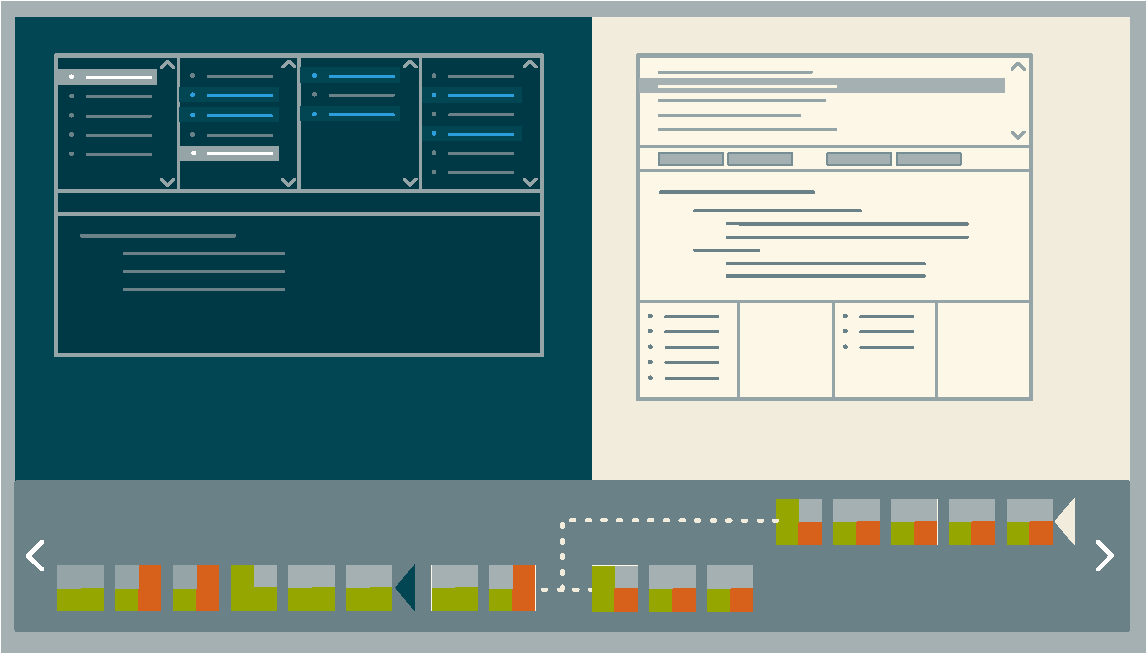
\includegraphics[width=\columnwidth]{figures/2_background/coexist2}
    \caption{Conceptual figure of CoExist featuring continuous
      versioning, running tests and recording the results in the
      background, and side by side exploring and editing of multiple
      versions.}
    \label{fig:CoExist}
\end{figure}

For that reason, CoExist preserves fast and easy access to previous
development states and information thereof~\cite{Steinert2012COE}.
For every change to the code base, CoExist creates a new
version. Users can rapidly switch versions or can access multiple
versions next to each other. CoExist thus gives users the impression
that development versions \emph{co-exist}. Fig.~\ref{fig:CoExist}
illustrates some of the main user interfaces concepts of CoExist.

With that, \coexist contributes the following concepts and tools:

\begin{description}
\item[Continuous Versioning] to create new versions in the background
  based on the structure of programs. It enables programmers to go
  back to a previous development state and to start over Starting over
  from a former development state, which will implicitly create a new
  branch of versions.
 
\item[User Interface Concepts] to support browsing and exploring
  version information as well as identifying a version of interest
  fast. CoExist provides two different concepts. First, it provides the
  version bar, which highlights version items that match the
  currently selected source code element. Hovering the items will
  display additional information such as the kind of modification, the
  affected elements, or the actual change performed. Second,
  programmers can use the version browser to explore information of
  multiple versions at a glance. The version browser displays basic
  version information in a table view, which allows to scan the
  history fast.

\item[Additional Environments] to explore static and dynamic
  information of previous development states next to the current set
  of tools.  Opening an addition environment is useful, when, for
  example, the programmer suddenly becomes curious about how certain
  parts of the source code looked previously or how certain effects
  were achieved. The additional environments also allow for running
  and debugging programs. With that, users are capable of efficiently
  recovering knowledge from previous versions, which avoids the need
  for a precise understanding of every detail before making any
  changes.

\item[Continuous and Back-in-time Analysis] for test cases and other
  computations. \coexist{} continuously runs analysis programs for
  newly created versions. As a default, it runs test cases to
  automatically assess the quality of the change made. The test result
  for a version are recorded isand presented in the corresponding item
  of the version bar (left of Figure~\ref{fig:CoExist}). The user can
  also run other analyses such as performance measurements. In
  addition to the continuous analysis features, CoExist provides full
  access to version objects and offers a programming interface to run
  code in the context of a particular version. So, whenever
  programmers become interested in the impact of their changes, they
  can easily analyze them in various respects. This allows programmers
  to ignore these aspects of programming at other times.

\item[Re-assembling of Changes] for sharing independent improvements
  in separate commits (Section~\ref{sec:re-assemble}). Users can
  extract selected changes to a new branch, test the result, and
  commit the achieved increment.
\end{description}

With CoExist, programmers can change source code without worrying
about the possibility of making an error. This is because they can
rely on tools that will help with whatever their explorations will
turn up. They no longer have to follow certain best practices in order
to keep recovery costs low.

Without CoExist, either compensational or precautionary actions are
necessary for recovery.  When programmers unintentionally introduce
errors, decrease performance, or harm the program design, they have to
repair changed code.  They either need to edit the code again or load
a previously commited version of the code.  Editing code of
potentially many methods across and many classes is obviously a
significant effort and error-prone.  Loading a previous version is
only possible if a version has been commited previously.  Therefore,
programmers can reduce the cost of recovery by anticipating recovery
needs beforehand.  However, preserving versions is also an effort and
especially so when revision histories are expected to be
well-documented and immediately useful.  For that, programmers need to
assemble changes to meaningful increments, run tests, and write
helpful commit messages.

CoExist, in contrast, makes recovery fast and easy.  So, instead of
worrying about negative consequences, programmers can focus on
implementing their ideas and rely on CoExist to help in case of
recovery needs.



\subsection{Part Development in Lively Kernel}
This subsection illustrates how Lively Kernel 

\subsubsection{The Lively Kernel and Morphic}
The Lively Kernel is a programming system in the tradition of
Smalltalk and Self.  Development happens at runtime.  It incorporates
tools and techniques to be completely self-sufficient.  Thus,
programmers can create versions of the Lively Kernel with the Lively
Kernel. The Lively Kernel is a browser-based system.  It is
implemented in JavaScript and renders to HTML.

The Lively Kernel implements Morphic~\cite{Maloney1995Mor}, a
framework for developing graphical applications.  The graphical
objects of this framework are called \emph{Morphs}. Each morph has a
class but can also have object-specific behavior. They can be created
by instantiating a class or by copying an existing morph. (Class-based
and prototype-based programming is mixed.) The copy operation does not
establish a prototypical inheritance relationship between the copy and
the original. Instead, it creates a full copy.

Programmers can change the position of morphs by \emph{dragging} and
the composition by an alternative dragging, called \emph{grabbing}.
When a morph is grabbed, it can be added to another morph and becomes
that morph's submorph.  This way, a morph does not have to be a basic
shape or simple widget, but can be the interface of any application.

\begin{figure}
    \centering
    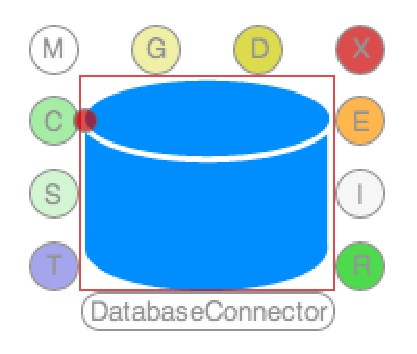
\includegraphics[width=0.3\columnwidth]{figures/2_background/1_halos.pdf}
    \caption{The halo buttons of a basic morph.}
    \label{fig:Halos}
\end{figure}

Morphs offer a set of manipulation tools called \emph{Halos}, as shown
in Figure~\ref{fig:Halos}.  Developers can bring up these tools for
each morph. Halos allow for directly manipulating morphs. Using halos,
users can resize, rotate, drag\&drop, and copy morphs. They can also
the directly change morph compositions ofby adding or removing morphs
as submorphs. Other halo buttons open tools such as an
\emph{Inspector}, \emph{Style Editor}, and \emph{Object Editor}. While
the inspector focuses on presenting all fields and values of each
object, the object editor provides means to browse and edit
object-specific scripts.

\begin{figure}
    \centering
    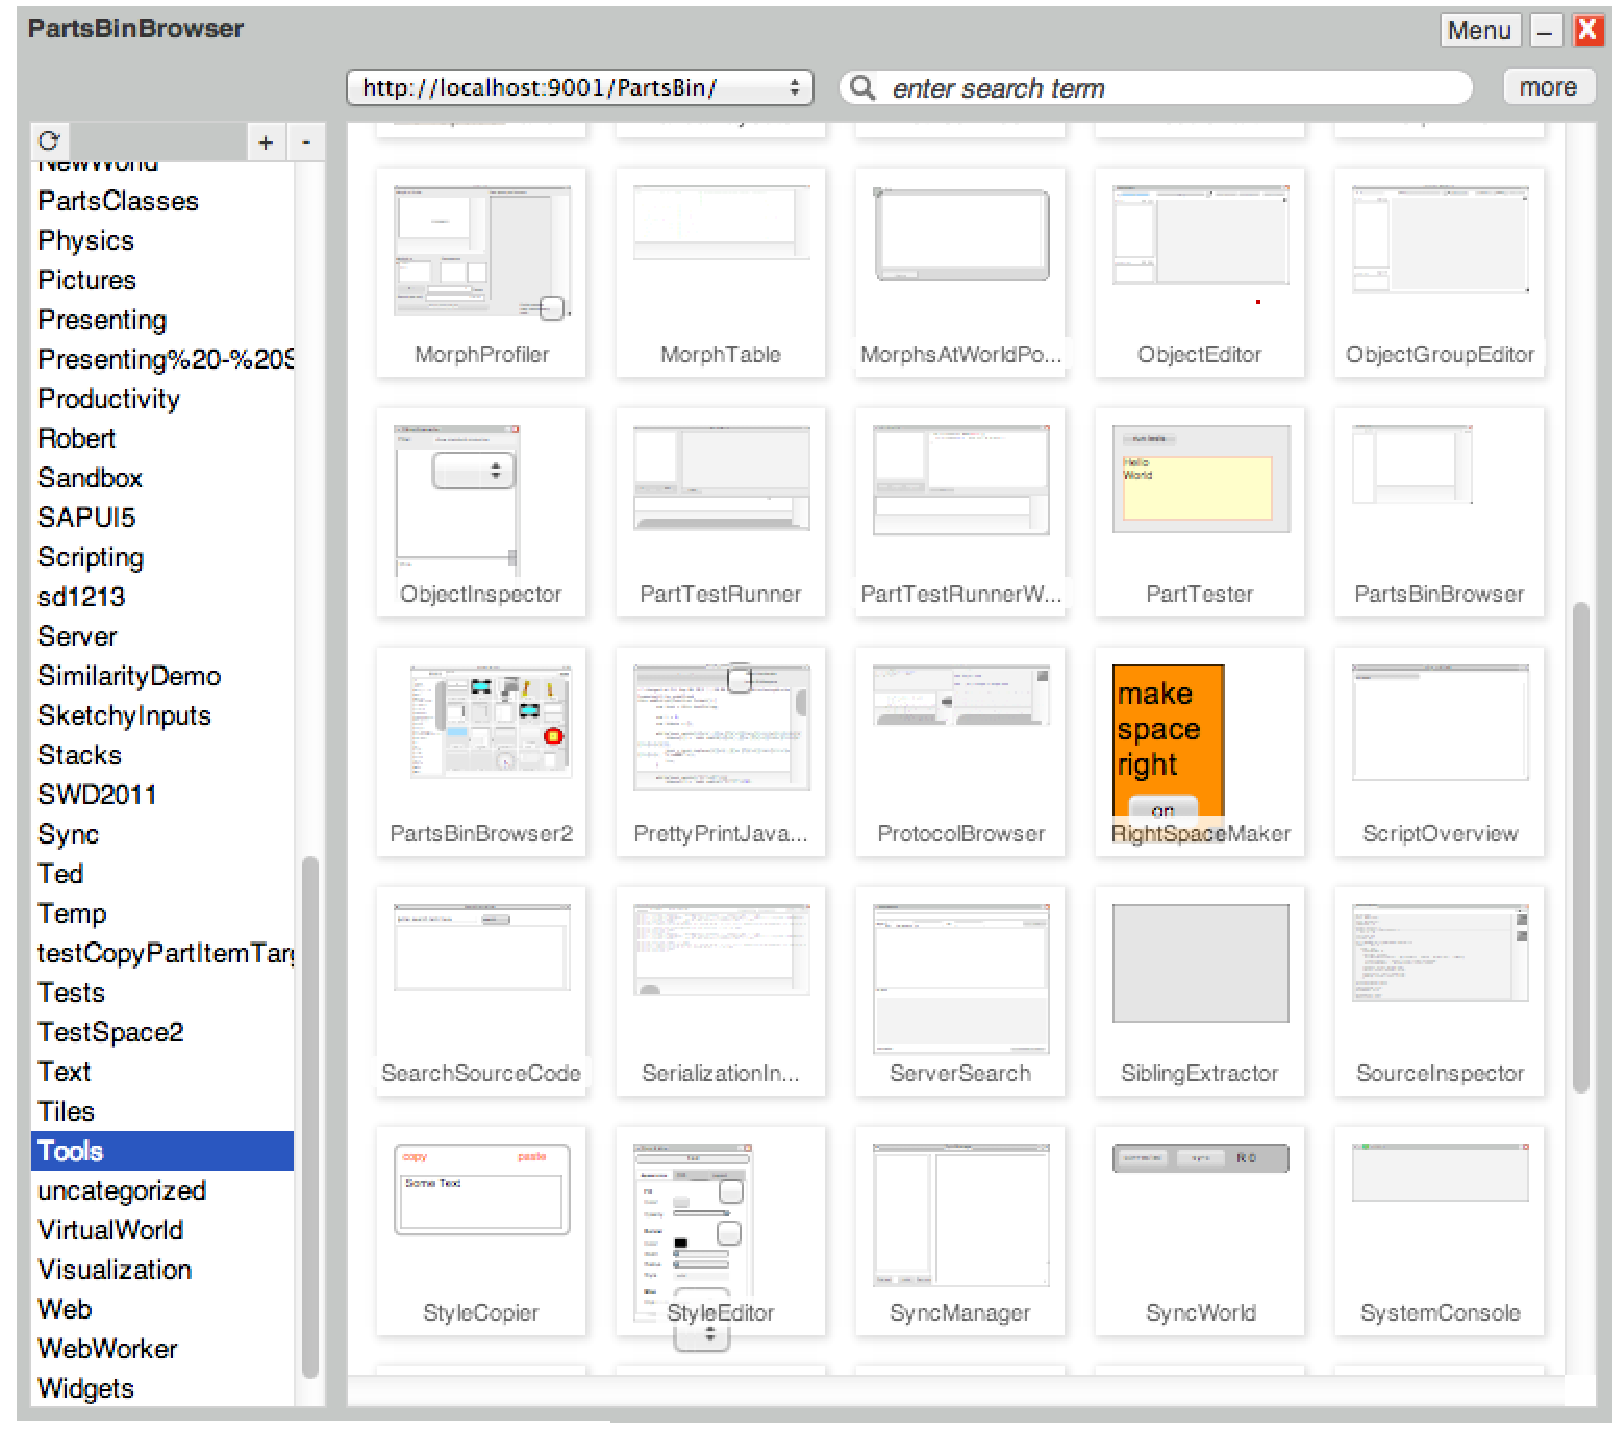
\includegraphics[width=\columnwidth]{figures/2_background/3_partsBin.pdf}
    \caption{The Lively Kernel's Parts Bin opened on the \emph{Tools} category.}
    \label{fig:PartsBin}
\end{figure}

Fig.~\ref{fig:PartsBin} shows Lively Kernel's \emph{Parts
  Bin}~\cite{Lincke2012LPC}, which is a repository of published morph
compositions called \emph{parts}. Users can use such published parts
for their own compositions and publish their creations to the
PartsBin. This way, various tools such as the Object Editor have been
created and made available this way.



\subsubsection{Part Development By Example}

To exemplify how developers work directly on objects in the Lively
Kernel, we will outline how a user adds a new feature to the Object
Editor.

In this example, the user adds a magnifier tool to the Object Editor.
The magnifier tool helps finding the editor's target, which is the
object the editor currently presents scripts for.  Implementing the
new feature requires to create a new button morph and to add it to the
editor, as shown in Figure~\ref{fig:MagnifierButton}.

\begin{figure}[h]
    \centering
    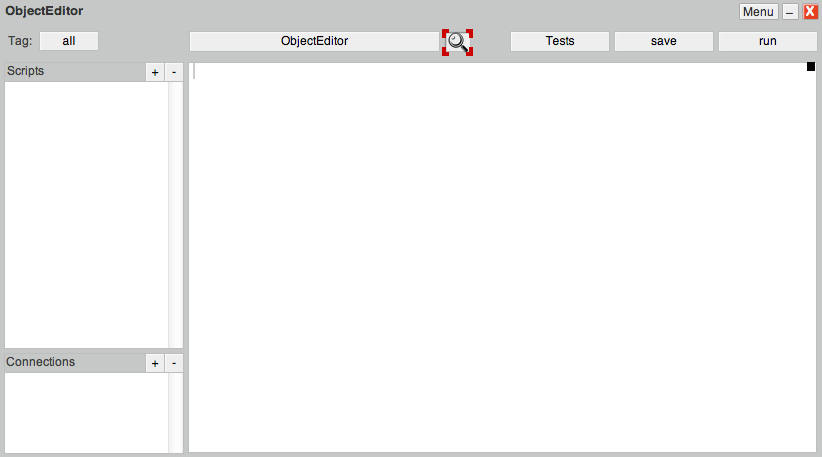
\includegraphics[width=0.7\columnwidth]{figures/3_motivation/1_magnifierButton.png}
    \caption{The Object Editor's magnifier button highlighted with a red outline.}
    \label{fig:MagnifierButton}
\end{figure}

The magnifier button has two features:

\begin{enumerate}
\item When a programmer hovers over the button, the Object Editor's
  current target is highlighted with a rectangular overlay.
\item When a programmer clicks the button, the current target
  selection is revoked and the programmer can select the new target of
  the editor.
\end{enumerate}

The following covers the first of the two features, which is also
shown in Figure~\ref{fig:MagnifierBehavior} for an Object Editor
currently targeting the character of a game.

\begin{figure}[h]
    \centering
    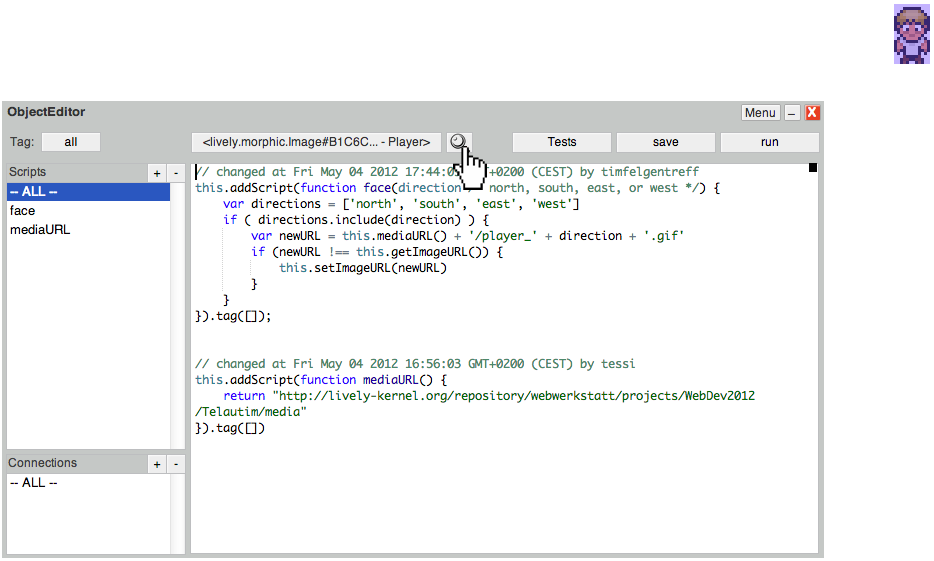
\includegraphics[width=0.8\columnwidth]{figures/3_motivation/2_magnifierBehavior.png}
    \caption{The Object Editor's magnifier button as it highlights the editor's target.}
    \label{fig:MagnifierBehavior}
\end{figure}

\paragraph{Manipulating the Button Morph}
Before implementing the button's behavior, the user first creates the
button and manipulates its visual appearance.
Figure~\ref{fig:ButtonBuilding} shows the steps in which the button is
manipulated.  A basic button, as visible in \circnum{1}, can be found
in the Parts Bin repository.  In \circnum{2}, the user resizes the
button and gives it a square extent using the \emph{Resize} halo
button.  Next, the user loads an image showing a magnifier icon.
Using drag and drop, the image is added to the button in \circnum{3}.
Dropping a morph onto another connects the two morphs.  Moving the
button around will then move the image accordingly.  Finally, the
users adds the result of these manipulations, visible in \circnum{4},
to the Object Editor.

All these changes are made directly to the state of objects: the
button morph, the magnifier image morph, and the editor morph.

When programmers edit parts in this way, they often see the effects of
their actions immediately.  For example, when adding the new button to
the Object Editor, the button is visible at all times.  Programmers do
not need to run any code to see and test the button.

\begin{figure}[h]
    \centering
    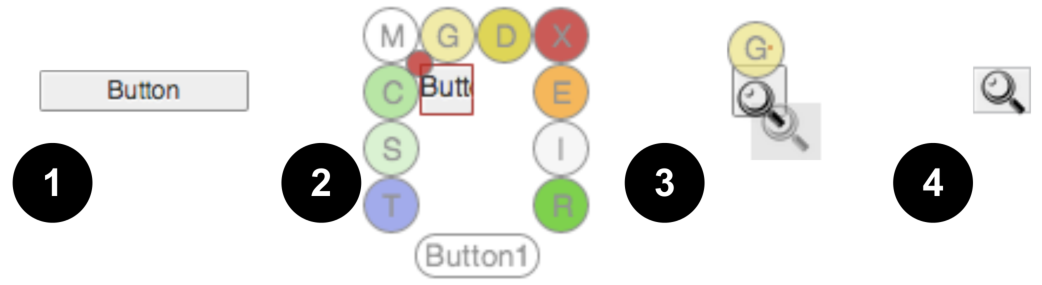
\includegraphics[width=0.8\columnwidth]{figures/3_motivation/3_buildingTheButton.pdf}
    \caption{Directly manipulating a button morph.}
    \label{fig:ButtonBuilding}
\end{figure}

\paragraph{Scripting the Button Morph}
Now the user implements the button's behavior.  The user adds scripts
to the button that lay a translucent rectangle over the current
target.  In particular, the button receives two scripts:
\lstinline{onMouseMove} and \lstinline{onMouseOut}.  The
implementation of the behavior includes the following:

\begin{itemize}
\item The button holds a semitransparent rectangle morph.
\item When the mouse enters the button (\lstinline{onMouseMove}), the
  button resizes and adds the rectangle to the Lively Kernel world at
  the position of the target.
\item When the mouse leaves the button (\lstinline{onMouseOut}), the
  button removes the rectangle from the world again.
\end{itemize}
 
The Lively Kernel's scripting tools allow to evaluate code in the
context of their target objects.  Hence, when programmers want to test
a script or even just specific lines of code, they can try the
behavior directly for the actual target.


\subsubsection{Recovery Needs When Developing Parts}

While manipulating objects directly, developers might make changes
which they later want to undo.

In the previous example the user could make \emph{accidental changes}:

\begin{itemize}
\item \textbf{Accidental changes to state}: The user could
  accidentally grap and move a morph such as the new button and,
  thereby, change a carefully arranged layout. Similarly, meaningful
  state can be lost when a morph, for example the new button, is
  accidentally removed from the world.
\item \textbf{Accidental changes to scripts}: The user could introduce
  a typographical error to or accidentally remove a script. Moreover,
  editing a script could introduce a defect or a decrease in
  performance.
\end{itemize}

Besides these accidental changes, well-intentioned changes can also
turn out to be \emph{inappropriate changes}:

\begin{itemize}
\item \textbf{Inappropriate changes through direct manipulation}: The
  user could make changes to the size, position, and colors of morphs
  to fine-tune the visual appearance of the editor's interface, only
  to decide later that a particular intermediate version was most
  appealing.
\item \textbf{Inappropriate changes through scripts}: The user could
  make a mistake in a workspace snippet that is intended to manipulate
  morph properties programmatically. Such a snippet can change many
  properties of many objects.
\end{itemize}

\paragraph{Explorative Script Evaluation}
Undesirable changes can also be introduced when a programmer explores
the behavior of objects by evaluating scripts.  The Object Editor
allows evaluating code directly for its target object.  While such
evaluation might help to understand the effects of particular code, it
might also change the state of objects.  For example, the user could
be working on the button's \lstinline{onMouseMove} script and could
evaluate a few lines of code to quickly test them.  These lines, as
shown in Figure~\ref{fig:onMouseOverScript}, would add the rectangle
to the editor's current target.  Only evaluating the selected lines
would, however, neither check the conditions usually checked above nor
set the state usually set below the selected lines.  Therefore,
evaluating this selection allows to test the highlighting behavior but
leaves the system in a state it normally would not be in.

\begin{figure}[h]
    \centering
    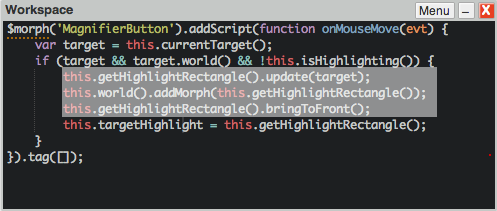
\includegraphics[width=0.7\columnwidth]{figures/3_motivation/4_workspaceDoIt.png}
    \caption{The button's \lstinline{onMouseMove} script with a text selection.}
    \label{fig:onMouseOverScript}
\end{figure}

The examples show that there are many situations in which the user
might want to undo previous actions.  In programming systems like the
Lively Kernel, where programmers work on objects, changes are always
made to the state of objects.  Functions are properties of objects.
Even classes and modules are objects.

For example, evaluating the text selection in
Figure~\ref{fig:onMouseOverScript} changes the \lstinline{world}
object's state.  The \lstinline{world} object has now one more
submorph, as shown in Figure~\ref{fig:changedCharacter}.  Thus, the
\lstinline{world}'s collection of submorphs is changed.

To undo the side-effect of the script and re-establish the previous
situation, the change to the \lstinline{world} object needs to be
undone.  The \lstinline{submorphs} property of \lstinline{world} has
to be as it previously was. When the state of all objects is
preserved and can be re-established, previous system states can be
recovered when necessary.

\begin{figure}[h]
    \centering
    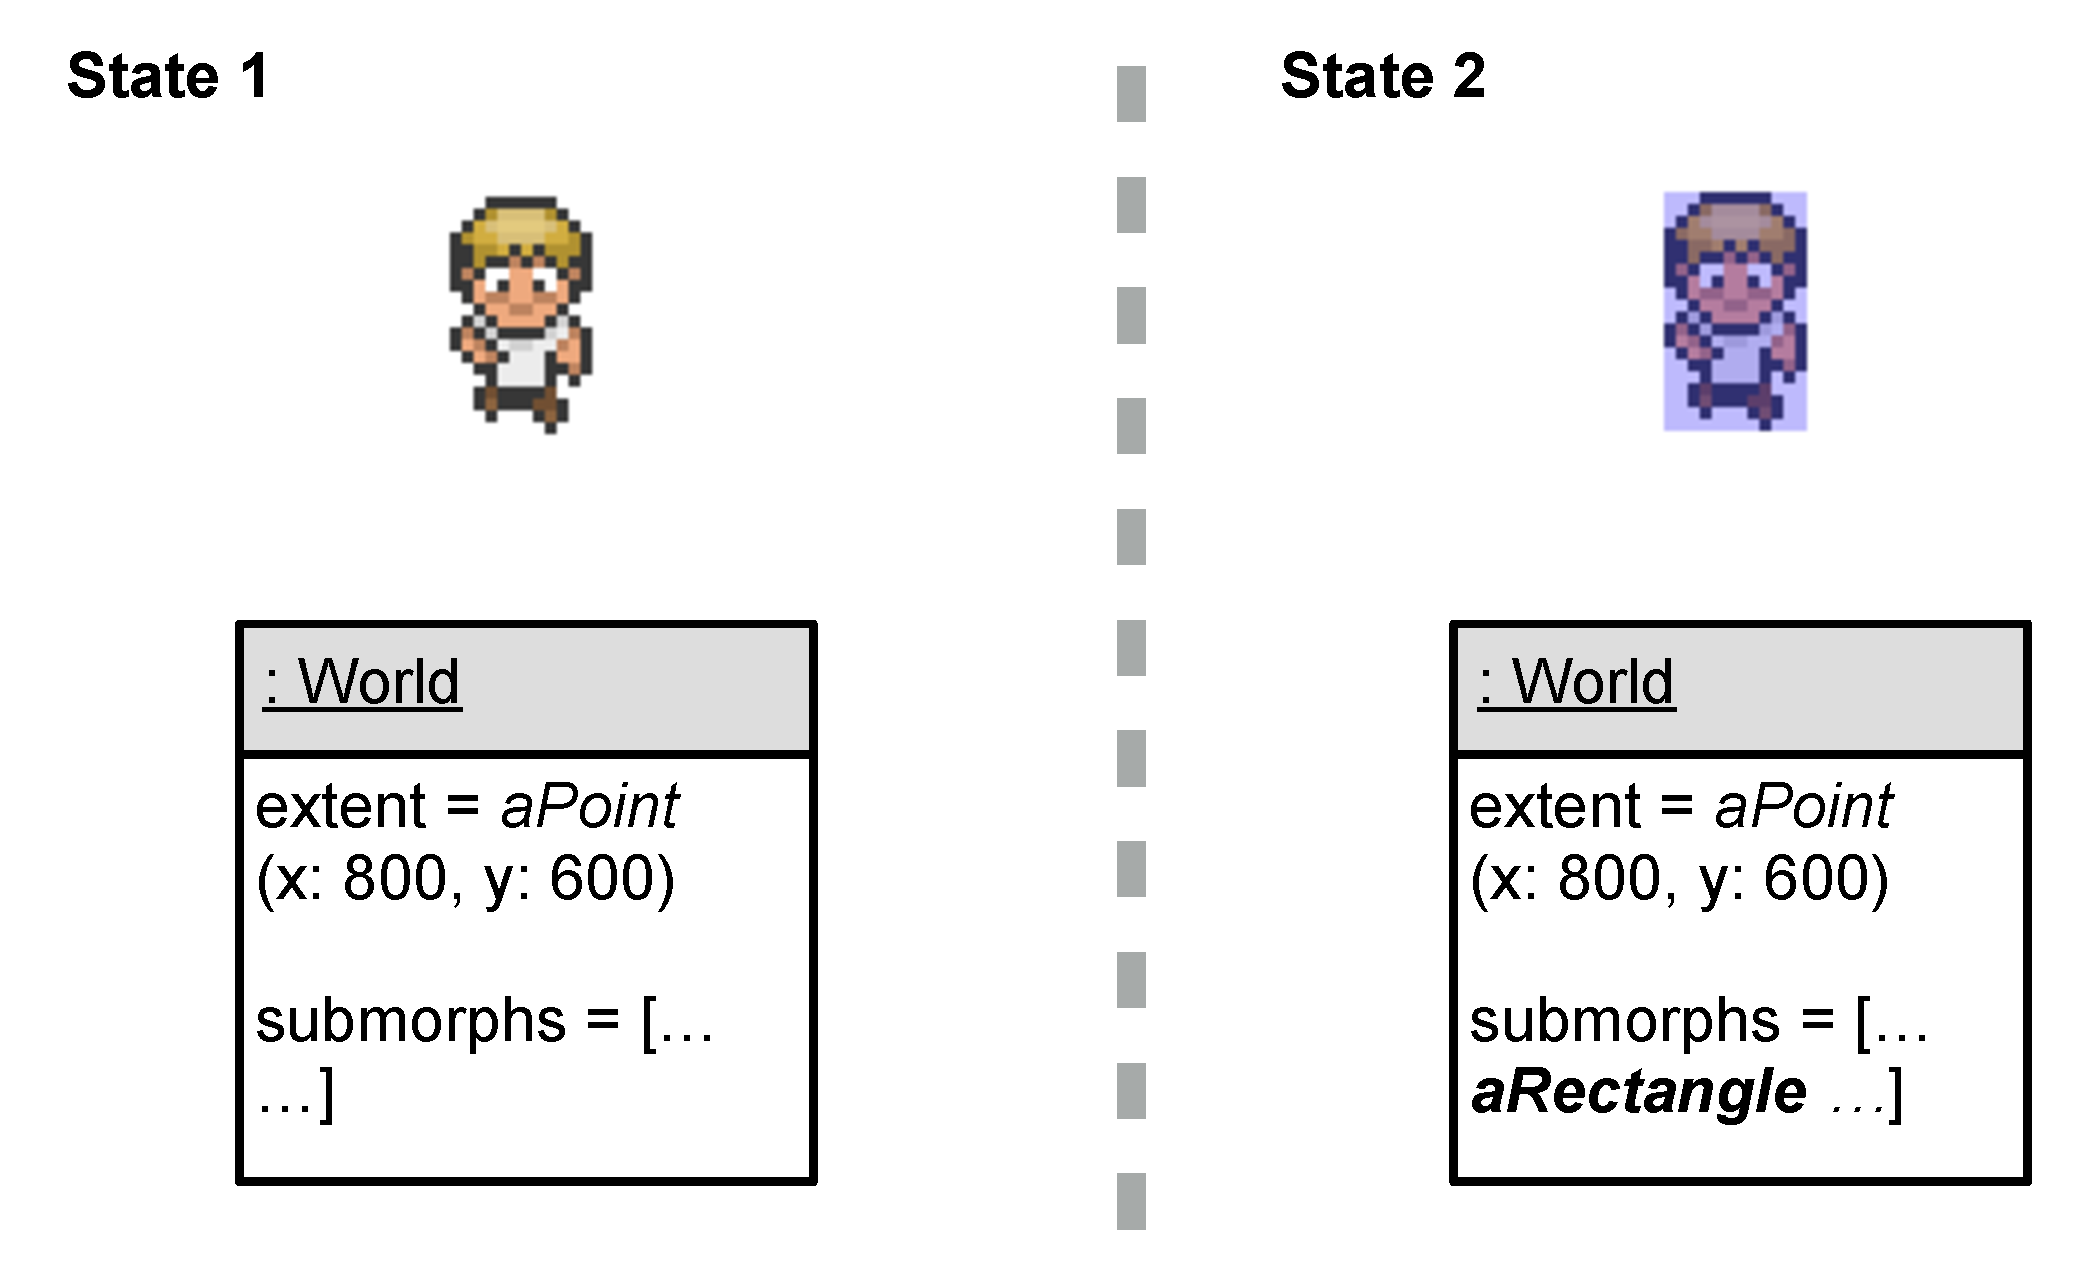
\includegraphics[width=0.6\columnwidth]{figures/3_motivation/5_stateChanges.pdf}
    \caption{Adding a submorph changes the state of a morph.}
    \label{fig:changedCharacter}
\end{figure}


%%% Local Variables:
%%% mode: latex
%%% TeX-master: "../main"
%%% End:
